\documentclass[smallextended]{svjour3}       % onecolumn (second format)

\usepackage{amsmath,amsfonts}  % AMS standard symbols and fonts
\usepackage{url}       % pretty clickable links
\usepackage{graphicx}  % including pictures
\usepackage{tabularx}  % center-aligned columns in table
\usepackage{mathtools} % "ceil" command
\usepackage{breqn}
\usepackage{color}

%
\def\UrlBreaks{\do\/\do-\do\_}

% Make line breaks occur on hyphens in URLs for BibTex.

% declare a "ceil" command
\DeclarePairedDelimiter{\ceil}{\lceil}{\rceil}

% correct bad hyphenation here
\hyphenation{op-tical net-works semi-conduc-tor}

%% Command for creating multiplie-line cells inside a table
\newcommand{\multilinecell}[2][c]{%
  \begin{tabular}[#1]{@{}c@{}}#2\end{tabular}}

% Declare title and authors
\title{Least Squares Solutions to Polynomial Systems of Equations with Quantum Annealing
\thanks{All authors contributed equally to this work. The author order was determined alphabetically.}}
\author{Tyler H. Chang \and Thomas C. H. Lux \and Sai Sindhura Tipirneni}

\titlerunning{LS Solution to Polynomial Systems}
\authorrunning{Chang, Lux, and Tipirneni}

\institute{T. H. Chang \at
   Virginia Polytechnic Institute and State University, Dept. of Computer Science, Blacksburg, VA, USA, 24061 \\
   \email{thchang@vt.edu}
   \and
   T. C. H. Lux \at
   Virginia Polytechnic Institute and State University, Dept. of Computer Science, Blacksburg, VA, USA, 24061 \\
   \email{tchlux@vt.edu}
   \and
   S. S. Tipirneni \at
   Virginia Polytechnic Institute and State University, Dept. of Computer Science, Blacksburg, VA, USA, 24061 \\
   \email{tsaisindhura@vt.edu}
}

\date{Received: date / Accepted: date}

\begin{document}

% Title area
\maketitle

% Abstract
\begin{abstract}
This work proposes and analyzes a methodology for finding least squares solutions to systems of polynomial equations.
Systems of polynomial equations are ubiquitous in computational science, with major applications in machine learning and computer security (i.e., model fitting and integer factorization).
The proposed methodology maps the squared error function for a polynomial equation onto the Ising-Hamiltonian model, ensuring that approximate solutions (by least squares) to real-world problems can be computed on a quantum annealer even when exact solutions do not exist. Hamiltonians for integer factorization and polynomial systems of equations are implemented and analyzed for both logical optimality and physical practicality on modern quantum annealing hardware.
\end{abstract}

\keywords{Least squares \and Quantum annealing \and Polynomial systems of equations \and Prime factorization \and Root finding}

% Body
\section{Introduction}

Quantum annealing (QA) provides a practical framework to realize adiabatic quantum computing (AQC), where AQC is a general purpose quantum computing framework that is known to be equivalent to the quantum gate model \cite{aharonov2008adiabatic}.
In the quantum gate model, quantum state vectors evolve through time via the application of quantum logic gates (unitary operators) \cite{steane1998quantum}.
On the other hand, AQC conceptually produces the solution to a problem through a single ``annealing'' operation.
This is achieved by transitioning from an initial Hamiltonian to an arbitrary Hamiltonian that encodes the problem, using the adiabatic theorem.
The standard implementation of QA only solves a subset of AQC problems because the allowed operators only span a subspace of all unitary operators.
Specifically, QA is limited to annealing over the span of the stoquastic Pauli-Z matrices, whose eigenstates are strictly real valued \cite{kadowaki1998quantum}.

While the general methodology for embedding classical programs in QA is understood, QA systems can still be tedious to program. D-Wave Systems has improved accessibility through its Ocean software suite that contains high-level programming modules for network science and constraint satisfaction problems.
Pakin also provides tools for embedding high-level constraint logic programs, using a standard cell library \cite{pakin2018performing}.
However, these approaches are inefficient for linear algebra and mathematical programming applications, making hand-crafted solutions preferred in many cases.
Linear algebra problems are ubiquitous in computational and data science, with some notable applications being least squares fitting, solving large sparse or dense systems, and even neural network training.
Such applications would certainly garner interest in high-profile fields such as machine learning, where the term ``quantum machine learning'' was coined by \cite{biamonte2017quantum}, and a quantum variational autoencoder is described in \cite{khoshaman2018quantum}.

In this work, a novel methodology is proposed for least-squares minimization of polynomial systems of equations via QA.
This broad class of problems is often referred to as sum of squares (SOS) polynomial minimization, and is a general case of both the least squares problem and the polynomial real-valued root-finding problem.
Solutions are obtained by mapping the squared error function for any multivariate polynomial onto a Hamiltonian embedding.
To make the proposed solution accessible, a high-level programming framework is provided, which automatically handles low-level details such as fixed-point binary encoding, quadratization, and both physical and logical (minor) embedding of the Ising-Hamiltonian model.
This framework is standalone, but interfaces with D-Wave's SAPI API.
One practical benefit of the squared error methodology is that the minimum forward error solution will correspond to the ground state for the Hamiltonian, and lower forward error solutions will have lower energies.
This causes the annealer to tend towards low energy solutions even when it fails to find the true global minimum.
Another benefit of both the methodology and the framework is that the fixed-point precision of each variable can be independently specified, and so this work immediately extends to nonlinear integer programming problems (such as integer factorization) and mixed-precision problems.

The remainder of this paper will proceed as follows.
Section 2 will present relevant background in QA, programming and algorithmic concerns, and related works.
Section 3 will introduce the proposed methodology for mapping multivariate polynomial systems of equations/SOS problems to the Ising-Hamiltonian model.
Section 4 contains a brief analysis of the proposed algorithm in terms of several performance concerns introduced in Section 2.
Section 5 contains technical details of the implementation, with a focus on the practicalities of the D-Wave machine.
Section 6 shows empirical results for $n$-bit integer factorization, least squares minimization of a system of polynomial equations, and solutions to linear systems of equations on the state-of-the-art D-Wave 2000Q quantum annealer.
Finally, Section 7 contains a conclusion and brief discussion.
\section{Background}
\label{sec:background}

At its foundation, QA utilizes the physical principle of quantum tunneling \cite{ray1989sherrington} to find grounds states for the Ising-Hamiltonian model
\begin{equation}
\mathcal{H}(\text{\boldmath$\sigma$}) = \sum_{i=1}^N h_i\sigma_i + \sum_{i=1}^N \sum_{j=i+1}^N J_{i,j} \sigma_i \sigma_j
\label{eq:hamiltonian}
\end{equation}
where $N$ denotes the number of qubits (quantum bits) involved in the computation (indexed $q_1,\ldots, q_N$), $\sigma_i \in \{-1,1\}$ denotes an eigenstate of $q_i$, $h_i$ denotes the bias of $q_i$, and $J_{i,j}$ denotes the coupler strength between the entangled pair $q_i$ and $q_j$.

Similarly as in AQC, QA achieves the solution to an arbitrary Hamiltonian by beginning from the ground state of an initial Hamiltonian $\mathcal{H}_0$, whose solution is known.
$\mathcal{H}_0$ is then gradually evolved through time into the problem Hamiltonian $\mathcal{H}_1$, via a mathematical homotopy of the form 
\begin{equation}
\mathcal{H}_s(\text{\boldmath$\sigma$}) = (1-s)\mathcal{H}_0(\text{\boldmath$\sigma$}) + s\mathcal{H}_1(\text{\boldmath$\sigma$}).
\label{eq:homotopy}
\end{equation}
Here, the time dependent variable $s$ transitions from $0$ to $1$ during the annealing time \cite{albash2018adiabatic}.

If the transformation (\ref{eq:homotopy}) is adiabatic, meaning that the surrounding temperature is near absolute zero and the rate of change in $\mathcal{H}_s(\text{\boldmath$\sigma$})$ is smaller than the energy gap $\Delta$ between the ground state of $\mathcal{H}_1$ and the next lowest energy eigenstate (i.e., the first excited state), then this process results in a solution to $\mathcal{H}_1$ with probability one.
Consequently, the annealing time $T$ required to find a true ground state with high probability is proportional to $\mathcal{O}(\Delta^{-2}|\log \Delta|^{6\alpha})$ \cite{elgart2012note}, where $\alpha$ is a Gevrey index, which describes the smoothness of the transition.
Rather than increasing the annealing time $T$ (approximately) quadratically as $\Delta$ shrinks, a more practical approach is to fix $T$ and instead increase the number of samples (i.e., runs of QA).
The probability of not achieving the ground state for {\it any} of the runs decreases exponentially with repeated independent samples, while the probability of a single anneal resulting in the ground state decreases quadratically with a decaying $\Delta$ \cite{kadowaki1998quantum}.
As a result, an exponentially decaying $\Delta$ only requires linearly increasing the number of samples to achieve the same likelihood of a ground state solution \cite{jiang2018quantum}.

Minimization of an arbitrary Ising-Hamiltonian is classically NP-complete \cite{barahona1982computational}, and although QA currently remains less efficient than classical heuristic techniques (such as simulated annealing), both theory \cite{santoro2002theory} and empirical research \cite{boixo2014evidence} suggest that QA will eventually overtake classical techniques as the preferred method for minimizing Ising-Hamiltonian equations.
Currently, the state-of-the-art in QA is pioneered by D-Wave systems, which produces both hardware and software for minimizing (\ref{eq:hamiltonian}) via QA.
The current flagship D-Wave machine is capable of performing QA with over 2000 qubits sparsely connected according to the Chimera graph topology, in which each qubit is connected to at most 6 other qubits. 
The next generation of machines will support QA with over 5000 qubits on a new Pegasus connection topology \cite{boothby2018next}, in which each qubit is connected to at most 15 other qubits.

D-Wave's QA hardware does not implement perfect adiabatic evolution and must account for real world practicalities such as outside noise, bias leakage, and short annealing times.
Therefore, it is useful to differentiate between the logical and physical Hamiltonians.
The {\it logical} Hamiltonian (often referred to in literature as the minor embedding) will be a functional of the form (\ref{eq:hamiltonian}), where $h_i$ and $J_{i,j}$ are real numbers.
Note that not all logical Hamiltonians can be embedded on a current D-Wave machine.
D-Wave requires that $h_i \in [-2,2]$, requires that $J_{i,j}\in[-1,1]$, uses a quantization step size of approximately $0.01$, and only allows for nonzero couplings between qubit pairs $q_i$ and $q_j$ that are connected according to some graph topology $G$ \cite{karimi2019practical}.
Therefore, it is important to distinguish the {\it physical} Hamiltonian as shown below, which could be implemented on the current D-Wave hardware.
\begin{equation}
\Tilde{\mathcal{H}}(\text{\boldmath{$\sigma$}}) = \sum_{i'=1}^{N'}\Tilde{h}_{i'}\sigma_{i'} + \sum_{(i',j') \in G} \Tilde{J}_{i',j'} \sigma_{i'} \sigma_{j'}
\label{eq:physical}
\end{equation}
Here, $N' \geq N$ is the number of physical qubits required to synthesize all the required connections through the ``chaining'' process, as shown in Figure \ref{fig:chains}.
After the chaining process is completed, the entire Hamiltonian is rescaled by some factor $\kappa$, which is the largest factor such that all resulting $\Tilde{h}_{i'} \in [-2,2]$ and $\Tilde{J}_{i',j'} \in [-1,1]$.
D-Wave provides embedding tools, which use heuristics to construct the chains and compute the corresponding constant $\kappa$.

Due to physical hardware limitations, such as the quantization step size, manufacturing imperfections, outside noise, and bias leakage, the problem solved by the D-Wave annealer is generally not identical to the physical Hamiltonian in (\ref{eq:physical}).
Rather, the D-Wave solves a perturbed model, as shown below.
\begin{equation}
\hat{\mathcal{H}}(\text{\boldmath$\sigma$}) = \sum_{i'=1}^{N'} (\Tilde{h}_{i'} + \delta_{i'})\sigma_{i'} + \sum_{(i',j')\in G} (\Tilde{J}_{i',j'} + \delta_{i',j'}) \sigma_{i'} \sigma_{j'}
\label{eq:perturbed}
\end{equation}
The problem (\ref{eq:perturbed}) will have the same ground state as (\ref{eq:physical}) if $\|\Tilde{\mathcal{H}} - \hat{\mathcal{H}}\|_\infty \leq \Delta'$, where $\Delta'$ is the size of the energy gap between the ground and first excited state of $\Tilde{\mathcal{H}}$, and $\|\cdot\|_\infty$ denotes the $H_\infty$ operator norm.
Note that the ratio $\|\Tilde{\mathcal{H}} - \hat{\mathcal{H}}\|_\infty/\Delta'$ can be considered analogous to the conditioning of the problem in this context.


\begin{figure}
\centering
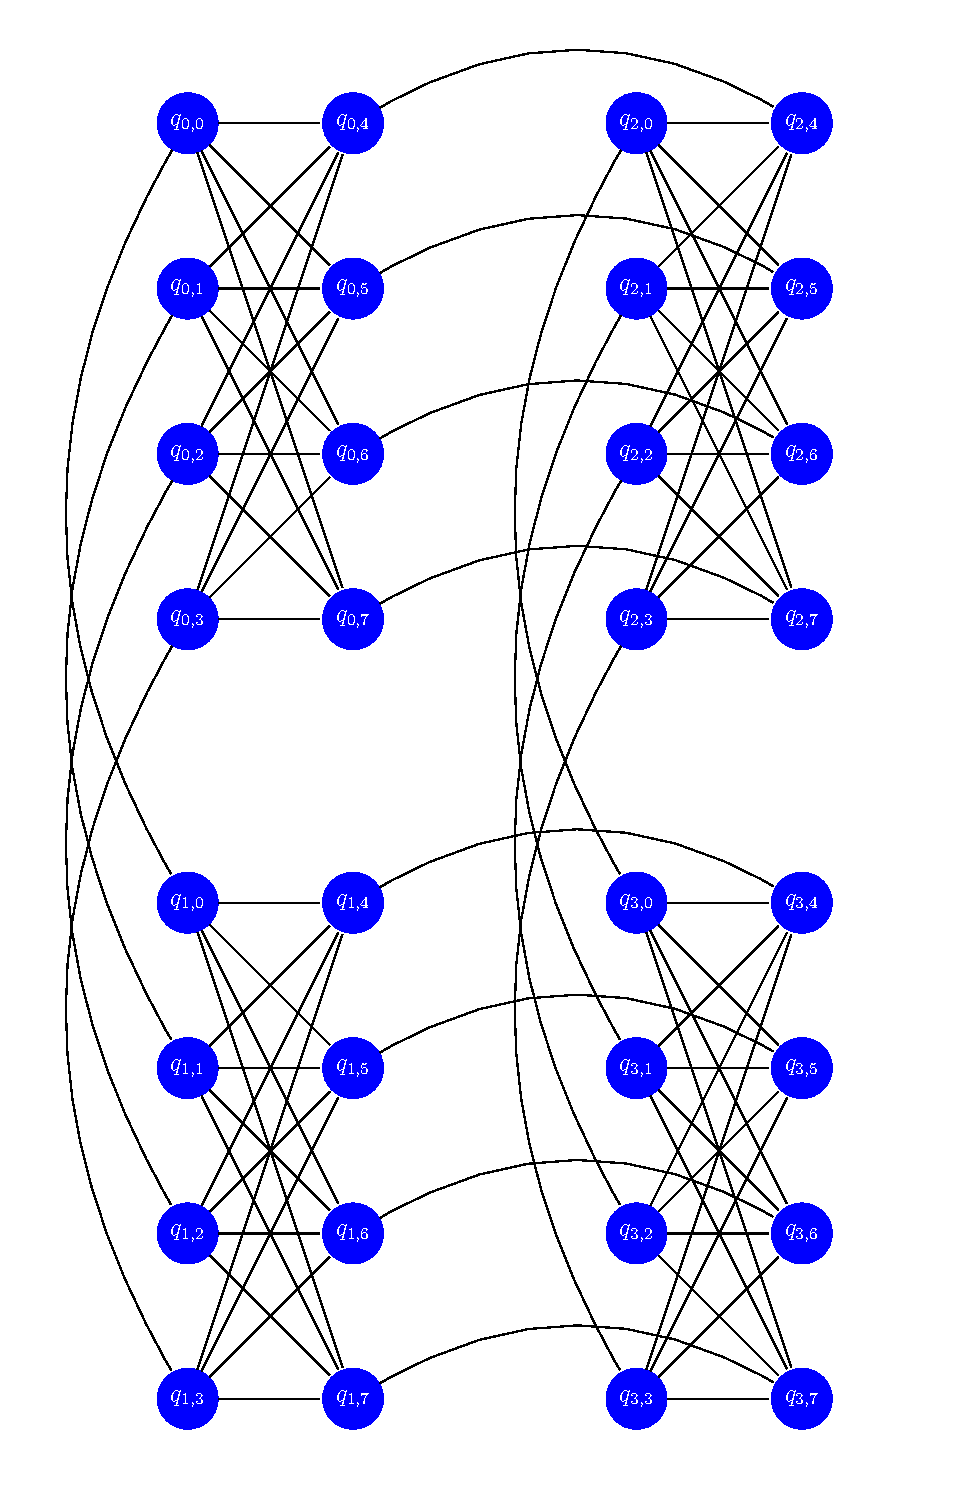
\includegraphics[width=0.45\textwidth]{fig1a.pdf}$\qquad$
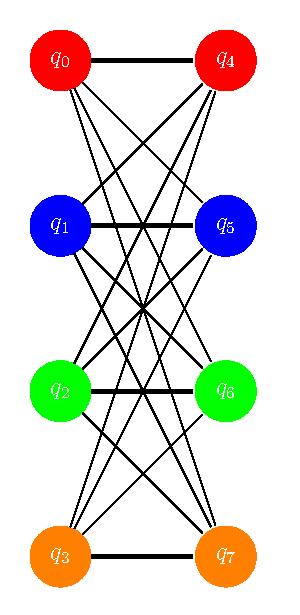
\includegraphics[width=0.35\textwidth]{fig1b.pdf}
\caption{Finding a physical embedding: this figure shows a toy 32 qubit system demonstrating the Chimera graph structure (left) and a synthesized dense network on an individual unit cell (right). The Chimera graph consists of bipartite 8-qubit unit cells as shown, with sparse connections between cells.
To synthesize a dense 4-qubit network on any individual unit cell, negative coupler weights (shown in bold) are added.
I.e., $J_{0,4} = J_{1,5} = J_{2,6} = J_{3,7} < 0$.
}
\label{fig:chains}
\end{figure}

To measure the optimality of an implementation, it is typical to consider both the number of physical qubits $N'$ required to embed the Hamiltonian and the size of the physical energy gap $\Delta'$.
In general, to implement a classical circuit on a QA machine, the circuit must be transformed into a Hamiltonian whose ground states correspond to valid input/output combinations as illustrated in Figure \ref{fig:xor-ex}.
During this process, it is common to introduce ancillary qubits, which are important terms in the Hamiltonian, but do not contain any useful information on input or output.
Using basic gates generated via the above process, it is possible to implement general classical circuits using the additive property of Hamiltonians \cite{pakin2018performing}.
While this methodology is convenient, it is wasteful in terms of ancillary bit requirements, and therefore a hand-crafted solution is preferable for most problems.

\begin{figure}
\centering
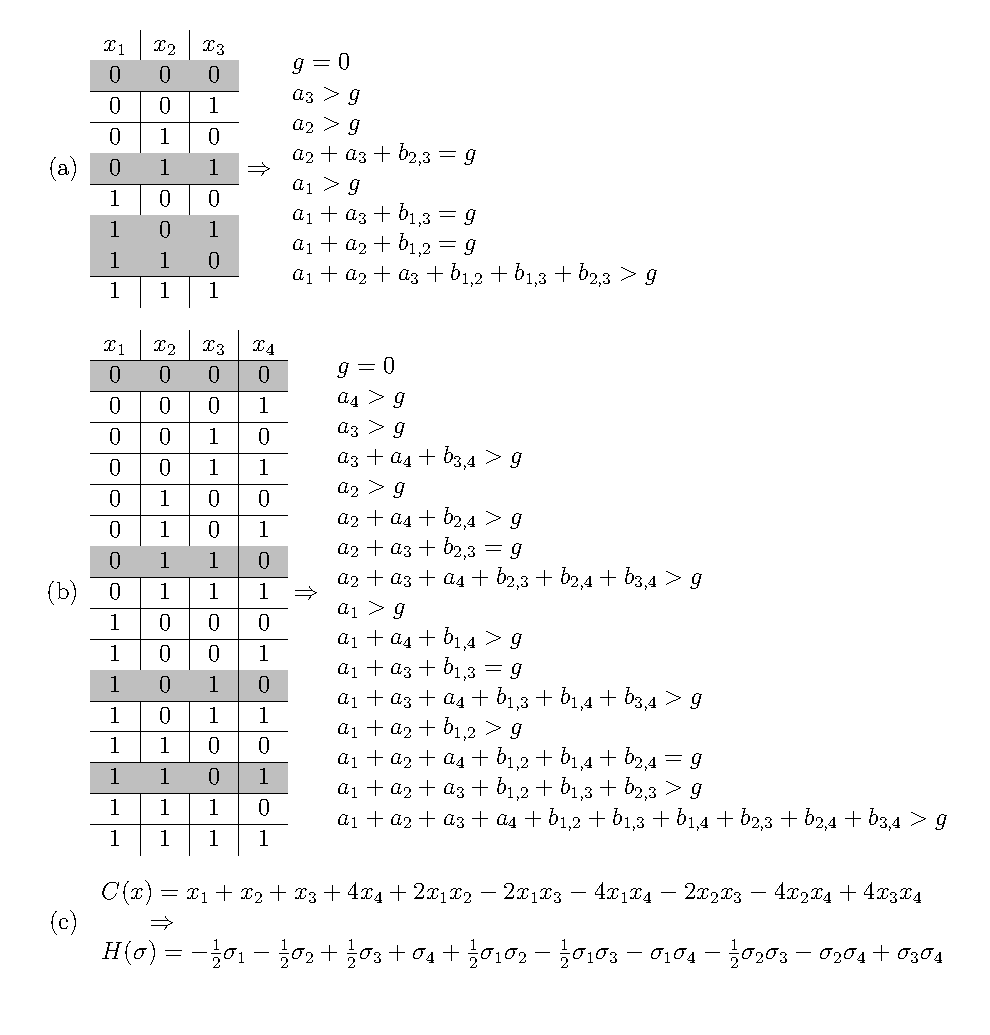
\includegraphics[width=0.9\textwidth]{fig2.pdf}
\caption{Embedding a quantum XOR gate: this figure illustrates the process of programming a quantum annealer, by embedding an XOR gate. The goal is to implement the circuit $x_1 \oplus x_2 = x_3$.
The truth table in (a) shows all combinations of $x_1$, $x_2$, and $x_3$, with all 4 valid input/output combinations highlighted.
Using the QUBO model, this generates the algebraic system of inequalities shown on the right hand side, where $g$ denotes the ground energy of the system.
Because the row containing all zeros is a valid solution, $g$ must be $0$.
The system of inequalities for (a) has no solution, so an ancillary bit $x_4$ is introduced in (b).
There are $2^4$ ways to assign the value of $x_4$ for the $4$ valid states from (a), some of which produce solvable systems and some of which do not.
By trial and error, the rows highlighted in (b) produce a solvable system, shown on the right hand side.
Solving this system produces the QUBO shown in (c), and applying the isomorphism results in the Hamiltonian below.
}
\label{fig:xor-ex}
\end{figure}

Using the transformation $\sigma_i = 2x_i - 1$ and dropping constant terms (which offset the energy landscape, but do not affect the locations of the minima), the Ising model is isomorphic to the quadratic unconstrained binary optimization (QUBO) model
\begin{equation}
C(\mathbf{x}) = \sum_{i=1}^N a_i x_i + \sum_{i=1}^N \sum_{j=i+1}^N b_{i,j} x_i x_j
\label{eq:QUBO}
\end{equation}
where $x_i\in\{0,1\}$ are abstract binary variables, $a_i = 2\left(h_i-\sum_j J_{i,j}\right)$, and $b_{i,j} = 4J_{i,j}$.
For dealing with binary representations of fixed-point numbers, the QUBO model is more convenient and will be favored in Section 3.
However, for performance analyses (Section 4) it is more accurate to consider the Hamiltonian model, which better describes the physical embedding.

The general problem of finding a least squares solution to a system of polynomial equations is equivalent to globally solving a multivariate SOS polynomial minimization problem.
This class of problems should not to be confused with the class of polynomial least squares problems, which refer to the fitting of a polynomial to data by solving a linear least squares problem.
Since SOS problems are known to be NP-hard, classical solutions focus on iterating toward a solution by solving sequences of linear matrix inequality problems \cite{lasserre2001global}.
In the special case where the system of polynomial equations is consistent, the problem can often be efficiently solved using homotopy methods \cite{watson1997algorithm}.
In the special case of linear and least squares systems, these problems can be solved with cubic complexity using standard matrix factorization techniques \cite{golub2012matrix}.

It should be noted that the current generation of D-Wave machines are not capable of solving any meaningfully large SOS problems.
In fact, the elementary operation of multiplication/factorization is considered difficult for these D-Wave machines, due to the practical limitations of D-Wave's technology \cite{andriyash2016boosting}.
Related to some of the applications discussed, a good deal of work has been put into integer factorization, with a focus on security applications.
While Shor's algorithm has become synonymous with quantum factorization, quantum annealing requires a different model \cite{shor1999polynomial}.
Early work in quantum factorization was pioneered by Peng et al., who produced a general model for integer factorization \cite{peng2008quantum}.
Jiang et al.\ expanded on this work in the special case of biprime factorization \cite{jiang2018quantum}.
Dridi et al.\ proposed an alternative approach to biprime factorization using Gr\"{o}bner bases \cite{dridi2017prime}.
In general, to factor an $n$-bit binary integer, these approaches require $\mathcal{O}(n^2)$ qubits and result in an exponentially decaying physical energy gap $\Delta'$.
It is also worth mentioning a hybrid quantum-classical algorithm for nonlinear integer programming, proposed by Alghassi et al.\ \cite{alghassi2019graver}.

For the special case of solving systems of linear equations, quantum algorithms have been proposed for both the gate model \cite{PhysRevLett.103.150502} and AQC model \cite{PhysRevLett.122.060504,PhysRevA.99.012320} that achieve exponential speedup in cases where the associated matrix has a low condition number.
For QA, there are two closely related works that were recently published, both of which achieve a QA solution by embedding the error function in the Ising-Hamiltonian.
Borle et al. \cite{borle2019analyzing} propose this methodology for solving linear systems of equations and least squares problems, but refrain from analyzing higher-order systems.
Chang et al. \cite{chang2019quantum} propose this method for finding least squares solutions to general systems of polynomial equations, but use a slightly different binary encoding technique, where fixed-precision signed arithmetic is achieved via a linear transformation of unsigned binary integers. The present work accompanies \cite{borle2019analyzing,chang2019quantum} by providing both an extension to higher order systems and an easily accessible coding framework for solving arbitrary polynomial SOS problems on a QA system.
\section{Embedding Polynomials}

Let $\mathbf{v}\in\mathbb{R}^d$ and let $p(\mathbf{v})$ be a multivariate polynomial of finite degree.
The goal of this section is to find real-valued least squares solution to equations of the form $p(\mathbf{v}) = 0$.
To do so, define the squared error function
\begin{equation}
E(\mathbf{v}) = \left( p(\mathbf{v}) \right)^2.
\label{eq:single-error}
\end{equation}
If $p(\mathbf{v}) = 0$ has real-valued solutions, then minimizing $E(\mathbf{v})$ will produce an element of the solution set.
If $p(\mathbf{v}) = 0$ is not exactly solvable for $\mathbf{v}\in\mathbb{R}^d$, then minimizing $E(\mathbf{v})$ will produce a solution in the least squares sense.
Similarly, given a system of polynomial equations $p_1(\mathbf{v})=0$, $\ldots$, $p_m(\mathbf{v})=0$, the total SOS error is given by
\begin{equation}
E(\mathbf{v}) = \left(p_1(\mathbf{v})\right)^2 + \ldots + \left(p_m(\mathbf{v})\right)^2.
\label{eq:system-error}  
\end{equation}
This section will show how to encode $\mathcal{H}(\text{\boldmath$\sigma$}) = E(\mathbf{v}) + \tau$, where $\mathcal{H}(\text{\boldmath$\sigma$})$ is an Ising-Hamiltonian of the form (\ref{eq:hamiltonian}), $E(\mathbf{v})$ is of the form (\ref{eq:single-error}), and $\tau$ is a constant energy offset.
SOS errors of the form (\ref{eq:system-error}) can be implemented trivially by summing over the individual Hamiltonians corresponding to each equation in the system.
As will be shown, the following process considers binary number representations of \textit{any} fixed precision, including those with mixed-precision and integer-valued problems.

Let $x_i\in\{0,1\}$ be the bit value of the $i$th bit of $x$, let $e$ denote a fixed exponent, and let $s\in\{-1,1\}$ denote whether $x$ is signed or unsigned ($-1$ for signed variables and $1$ for unsigned variables).
Then the following equation defines an $n$-bit binary encoding of $x$ using two's complement for signed numbers and a fixed-point precision determined by the exponent $e$.
Note that choosing $e=0$ results in an integer-valued problem.
\begin{equation}
x = 2^e \Bigg ( \sum_{i=1}^{n-1} 2^{i-1} x_i + 2^{n-1}x_{n}s \Bigg )
\label{eq:binary-encoding}
\end{equation}
Now, let $\mathbf{v} = [x^{(1)}, \ldots, x^{(d)}]^T$ and combine (\ref{eq:single-error}) and (\ref{eq:binary-encoding}) to express the energy as a multivariate binary polynomial with real-valued coefficients.
To get a QUBO expression of the form (\ref{eq:QUBO}), terms with three or more interacting variables must be quadratized (reduced to two-local form).
Many quadratization methods exist \cite{dattani2019quadratization}, but all known methods that maintain the squared-error energy landscape (i.e. reproduce the ground state and the full spectrum) utilize ancillary qubits.
This work employs reduction by substitution \cite{rosenberg1975reduction} for its equivalence with the logical AND operation.
The accompanying AND QUBO enforces $z_3 = z_1 \wedge z_2$ by assigning weights
\begin{equation}
C_{\wedge}(\mathbf{z}) = 3z_3 + z_1 z_2 - 2 (z_1 z_3 + z_2 z_3).
\label{eq:and}
\end{equation}

For example, consider the binary energy polynomial ${\tilde E}(\mathbf{x}) = x_1x_2x_3x_4$. Then setting $y_1 = x_1 \wedge x_2$ and $y_2 = x_3 \wedge x_4$ using (\ref{eq:and}) and summing over QUBOs gives 
$$
{\tilde C}(\mathbf{x},\mathbf{y}) = y_1y_2 + 3y_1 + 3y_2 + x_1x_2 + x_3x_4 - 2(x_1y_1 + x_2y_1) - 2(x_3y_2 + x_4y_2).
$$

When quadratizing terms as above, it is important to weight each occurrence of $C_\wedge$ by some large constant $\omega$ so that breaking an AND constraints incurs a large penalty.
Otherwise, the annealer could conceivably break an AND constraint to achieve an impossibly low squared error, resulting in a nonsensical solution.
As a rule of thumb, $\omega$ should be significantly greater than the expected squared residual but small enough so that $\Delta'$ is not unduly affected (as detailed in Section 4).
As long as the AND constraints are satisfied, the resulting QUBO will satisfy $C(\mathbf{x}) \cong E(\mathbf{v})$ and the resulting logical Hamiltonian will satisfy $\mathcal{H}(\text{\boldmath$\sigma$}) \cong E(\mathbf{v}) + \tau$, where the congruence is understood through the binary encoding of each $x^{(k)}$.

\section{Algorithm Analysis}

This section provides an overview and analysis of the important factors to consider when encoding polynomial systems of equations onto a quantum annealing architecture (resembling modern D-Wave hardware).

\subsection{Energy Gap}

The range of energies grows and shrinks exponentially with the bits of precision $n$, yielding a $\mathcal{O}(2^{-n})$ decay in the physical energy gap $\Delta'$ after the necessary rescaling operations.
When mixed-precision variables interact, $\Delta'$ is determined by the effective precision $\hat n$, which is the difference between the largest and smallest nonzero absolute value representable among all the variables in the system.
The number of additions $\alpha$ and number of multiplications $\mu$ have, respectively, linear and exponential effects on the maximum energy of the logical Hamiltonian.
Therefore, $\Delta'$ shrinks inverse linearly with respect to $\alpha$ and exponentially with respect to $\mu$.
Similarly as with addition, the number of equations $m$ in a system decreases $\Delta'$ at most inverse linearly since the equations do not directly interact, but may share some terms in common.
Combined, this yields a rate of decay for the physical energy gap (after rescaling) of
$$\Delta' \approx \mathcal{O}\bigg(\frac{1}{\alpha m 2^{\hat n \mu}}\bigg).$$
In general, it can be seen that $\Delta'$ will be primarily determined by the exponential decay $2^{-{\hat n}\mu}$.

\subsection{Number of Qubits}

Other than the number of qubits required to represent the binary numbers, some ancillary qubits may be introduced into the logical Hamiltonion during both quadratization and physical embedding.
Quadratization is performed analytically by the high-level tool described in Section 5, and so the ancillary qubit requirements due to quadratization can be easily analyzed.
When addition or subtraction is performed, no additional quadratization is required.
However, multiplication between two variables with $n_0$ and $n_1$ bits of precision requires $n_0 \times n_1$ ancillary qubits (one for each quadratization).
Given a maximum of $\mu$ multiplications per individual polynomial (single equation) and $n$ bits of precision, the number of ancillary qubits introduced through quadratization will be $\mathcal{O}(m n^\mu)$.
Notice that increasing the number of equations $m$ can at most linearly increase the number of ancillary quadratization terms required (when no variable products are shared between equations).
Also notice that the number of variables $d$ does not affect the number of ancillary qubits due to quadratization, for a fixed $\mu$.

When embedding the physical Hamiltonian for a polynomial system, two factors will dominate the number of necessary qubits.
First, the annealer must generate a fully connected subgraph of size $n^{(\mu + 1)/2}$.
Second, given some variable $\hat{\mathbf{x}}$ is multiplied by $k$ other distinct variables throughout a system, $\hat {\mathbf{x}}$ will have at least $k$ connections to each of its bits.
The modern Chimera graph structure is not conducive to fully-connected graphs nor small sets of qubits with high graph centrality, hence experimental results show a growth rate greater than $k n^\mu$ for large problems.

\subsection{Sensitivity to Perturbation}

Given the perturbed Hamiltonian model (\ref{eq:perturbed}), it is reasonable
to wonder how the perturbations $\delta_i$ and $\delta_{i,j}$ will affect
the quality of the solution.
In particular, one might wonder whether the effects could be great enough
so that the ground state of the perturbed problem is no longer the ground
state of the original problem.

Consider first an arbitrary physical Ising-Hamiltonian $\Tilde{\mathcal{H}}$ involving $N'$ physical qubits, as defined in (\ref{eq:physical}) and its corresponding perturbed Hamiltonian $\hat{\mathcal{H}}$ as in (\ref{eq:perturbed}).
Suppose that $|\delta_i|, |\delta_{i,j}| < \delta$, where $\delta>0$ is a constant that represents the largest magnitude perturbation possible on the current hardware.
Combining equations (\ref{eq:physical}) and (\ref{eq:perturbed}), applying the upper bounds $\delta$, and combining like terms yields
$$
\|\Tilde{\mathcal{H}} - \hat{\mathcal{H}}\|_\infty
= \sup_{\sigma} |\mathcal{H}(\sigma) - \hat{\mathcal{H}}(\sigma)|
\leq \sup_\sigma \left|\sum_{i'=1}^{N'} \delta \sigma_{i'} +
\sum_{i'=1}^{N'}\sum_{(i',j')\in G}\delta\sigma_{i'}\sigma_{j'} \right|.
$$

In the worst case, assuming nonzero connections between all physical qubits, the right hand side is upper bounded by $(N' + N' L')\delta$, where $L'$ is the number of connections per node in the physical graph $G$.
For the Chimera graph, each node has at most $6$ undirected edges.
So for the D-Wave Chimera architecture, the condition that guarantees a correct ground state for the physical Hamiltonian $\hat{\mathcal{H}}$ is $7N' \delta < 2\Delta'$.

\section{Experimental Methods}

For the results presented in Section 6, logical Hamiltonians were generated via the process described in Section 3 and run on a D-Wave 2000Q machine.
Before performing quadratization or constructing the logical chains, the initial rescale factor $\lambda_I$ necessary to encode the logical Hamiltonian weights into the range allowed by the physical Hamiltonian was computed.
For all demonstrations the AND weights used for quadratization were set to $\lambda_I / 8$, with $1/8$ being the largest power of 2 multiplier that yields correct solutions on all test problems.
After adding the AND gates to the logical Hamiltonian, the final rescale factor $\lambda_F$ necessary to encode the physical Hamiltonian was computed and the chain strengths were set to $\lambda_F$.
Finally, the {\verb minorminer.find_embedding } tool from D-Wave's Ocean toolkit was used to construct the logical chains and perform the necessary rounding, completing the physical embedding \cite{cai2014practical}.
Any chain breaks were resolved by majority vote, and similarly, any violated AND gates were corrected in a post-processing step.
For each run, the default annealing time of 20 microseconds is used, along with D-Wave's default annealing schedule.

\subsection{Code Availability}

Python code with a user-friendly interface has been produced that automates the process for generating QUBOs, handles AND gate and chain weighting, generates physical Hamiltonian embeddings, runs on either simulated or physical hardware, and resolves AND gate and chain breakage.
Each of these steps is carried out exactly as described above.
This code library was used for generating the Hamiltonians in the Results section and is available on GitHub at \url{https://github.com/tchlux/qaml}.
Note, the library uses the SAPI API, and therefore depends on several D-Wave toolkits for finding physical embeddings on the Chimera graph structure and accessing D-Wave's cloud QA solvers.
The exact code used for replicating the experiments and the corresponding data for Tables \ref{tab:biprime}, \ref{tab:poly_ls}, and \ref{tab:linear_ls} are located in the {\verb qaml/experiments } subdirectory.
It is worth noting how concisely the following experiments are implemented in the provided framework (just 5, 7, and 14 lines of code for experiments 6.1, 6.2, and 6.3, respectively), as the high-level abstractions are conducive to programming and solving arbitrary polynomial systems on a quantum annealer with ease.

\section{Results}

In this section, Hamiltonian embeddings for error functions of the form (\ref{eq:single-error}) and (\ref{eq:system-error}) are implemented for solving biprime factorization, polynomial SOS problems, and linear systems of equations.
For the first two problem, the focus is placed on increasing the bit precision $n$, since
it was shown in Section 4 that increasing the relative precision causes the physical energy gap $\Delta'$ to decay exponentially.
For problems with $n$ bits of precision per variable, the number of samples was assigned to $500n$ (a linear increase).
As outlined in Section \ref{sec:background}, this should maintain a (nearly) constant probability of achieving the ground state under ideal conditions.
However, since the problem conditioning is largely determined by $\Delta'$, it is somewhat concerning that the perturbations in (\ref{eq:perturbed}) could have a significant negative impact on the computation for large precision $n$.
In fact, the problem conditioning does seem to cause some significant decay in the probabilities.
However, the presented results achieve the ground state for every problem that could be embedded on the current D-Wave hardware, indicating that the primary limiting factor is the number of physical qubits $N'$ required to embed the physical Hamiltonian.

For the linear system problem, the focus is shifted to how the proposed methodology is affected by increasing the number of equations and variables, with a fixed four-bit precision.
Since there is no multiplication between variables in a linear system, the analysis results of Section 4 suggest that these types of problems should scale better on the D-Wave 2000Q hardware.
However, somewhat surprisingly, the D-Wave is unable to find exact solutions for relatively small linear systems, even when the true solution is exactly representable for the binary encoding.

\subsection{Factorization}
\label{sec:factorization}

To factor a biprime $M = x^{(1)}x^{(2)}$, where $x^{(1)}$ and $x^{(2)}$ are $n$-bit unsigned integers, the corresponding polynomial is 
$$
p\left(x^{(1)},x^{(2)}\right) = x^{(1)}x^{(2)} - M
$$
and the squared error function is given by
\begin{equation}
E\left(x^{(1)},x^{(2)}\right) = \left(x^{(1)}x^{(2)} - M\right)^2.
\label{eq:primefact}
\end{equation}
Creating $n^2$ ancillary qubits $y_{i,j} = x^{(1)}_i \wedge x^{(2)}_j$, this energy function can be embedded into a QUBO as described in Section 3.
Note that the best available techniques also require $\mathcal{O}(n^2)$ ancillary qubits for prime factorization \cite{dridi2017prime,jiang2018quantum,peng2008quantum}. 
The results for embedding this QUBO as a physical Hamiltonian (as described in Section 5) and running on the D-Wave hardware are shown in Table \ref{tab:biprime}.
Similar to the work done by Jiang et al.\ for biprime factoring, this methodology encodes $M$ directly into the Hamiltonian as a constant, rather than wasting extra qubits to store $M$ as a variable.
In fact, Jiang et al.\ used a nearly identical methodology for arbitrary integer factorization, but favored a multiplication table for factoring biprimes.


\begin{table}
    \centering
    \begin{tabular}{c|c c c|c c|c|c}
         Bits & $x^{(1)}$ & $x^{(2)}$ & $x^{(1)}x^{(2)}$ & Logical & Physical & Sq. Error & Occurrence \\ \hline
         2 & 2 & 3 & 6 & 8 & 16 & 0 & 180 \\
         3 & 5 & 7 & 35 & 15 & 69 & 0 & 311 \\
         4 & 11 & 13 & 143 & 24 & 148 & 0 & 35 \\
         5 & 29 & 31 & 899 & 35 & 349 & 0 & 82 \\
         6 & 59 & 61 & 3599 & 48 & 658 & 0 & 7 \\
         7 & 113 & 127 & 14351 & 63 & 1293 & 0 & 3 \\
         8 & 241 & 251 & 60491 & 80 & -- & -- & -- \\
    \end{tabular}
    \caption{Using the squared-error energy function methodology, biprimes with various bits of precision are factored. The columns depict the number of bits, the numbers multiplied and their product, the number of logical and physical qubits required, the minimum squared error (minimum energy) achieved by the quantum annealer, and the number of samples that produced the optimal solution. The number of samples taken grows as $500n$, where $n$ is the number of bits. Correct solutions are found for all embedded problems, however at 8-bits no physical embedding could be discovered for the logical Hamiltonian on the available the hardware. The multiplication circuit constructed with this methodology has a dense $n^2$ subgraph as well as a dense $n$ subgraph, making the number of physical qubits required to embed the Hamiltonian grow faster than the number of logical qubits on the Chimera graph structure of the available quantum annealing hardware.}
    \label{tab:biprime}
\end{table}

The most recent work in biprime factorization solves a slightly larger problem \cite{dridi2017prime,jiang2018quantum} by assuming properties of the factors.
In contrast, this methodology can factor arbitrary integers (which may not be biprimes) while still achieving the same number of bits of precision as those best known results.
As presented, arbitrary integer factorization takes the same form as biprime factorization, but has more candidate solutions (and an innately higher likelihood of success).
For that reason, only biprimes are considered here.
The correct factorization is obtained up to $M=14351$ (whose prime factors are both $7$-bit unsigned integers) by minimizing (\ref{eq:primefact}), which is also the largest problem that can be successfully embedded on current quantum annealing hardware.
At $n=8$ bits of precision, the Hamiltonian failed to embed onto the D-Wave 2000Q system, due to size limitations.

\subsection{Nonlinear Least Squares}


\begin{figure}
\centering
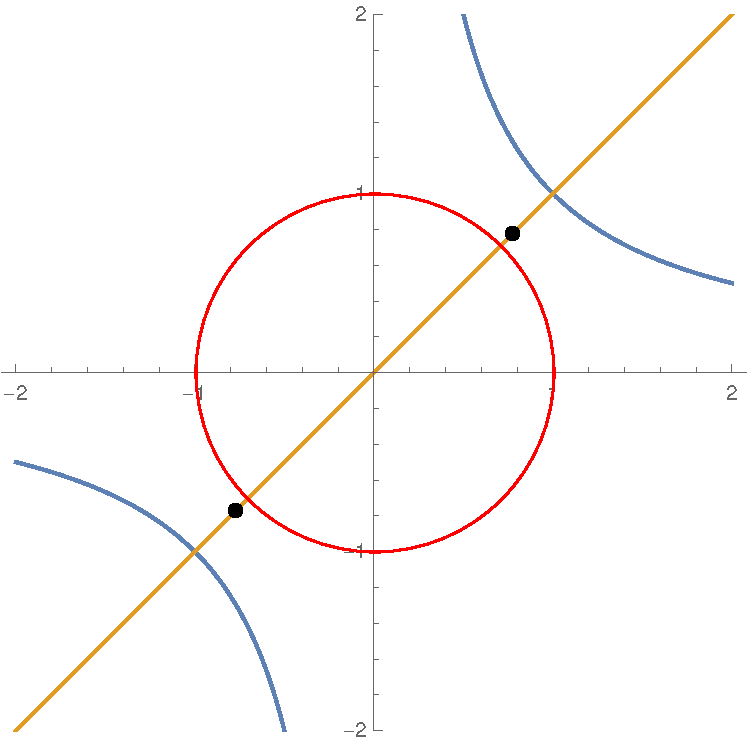
\includegraphics[width=0.9\textwidth]{fig3.pdf}
\caption{Least squares graph: this figure shows a plot of the least squares problem defined by the polynomial system of equations $xy=1$, $x^2 + y^2 =1$, and $x-y=0$.
The solutions of $(0.7746,0.7746)$ and $(-0.7746,-0.7746)$ are shown.
}
\label{fig:ls-graph}
\end{figure}

Let $\mathbf{v} = [x,y]^T \in \mathbb{R}^2$, and consider the following system of polynomial equations.
\begin{equation}
\begin{array}{rcl}
    xy &=& 1\\
    x^2+y^2 &=& 1\\
    x - y &=& 0
    \end{array}
    \label{eq:ls-system}
\end{equation}
This results in the squared energy function
$E(\mathbf{v}) = (xy-1)^2 + (x^2+y^2 - 1)^2 + (x-y)^2$.
A graph of the system (\ref{eq:ls-system}) is shown in Figure \ref{fig:ls-graph}.
To find the solution in the first quadrant, $x$ and $y$ are encoded as unsigned $n$-bit numbers each with an exponent of $e = -n$ using the encoding (\ref{eq:binary-encoding}).
The true solution is $x=y\approx 0.77$, with a minimum squared residual of $r^2 = 0.2$.
For $n=2$, the physical embedding is shown in Table \ref{tab:poly_ls_embedding}.
As seen in Table \ref{tab:poly_ls}, for $n>2$, the physical qubit requirement appears to grow super-linearly but sub-exponentially with the logical qubit requirement.

\begin{table}
    \centering
    \begin{tabular}{c|c c c|c}
      Logical Bit & Embedding &$\quad$& Logical Bit & Embedding \\ \cline{1-2}\cline{4-5}
      1 & 1376, 1383, 1248 && 6  & 1390, 1382, 1384 \\
      2 & 1380, 1379, 1251 && 7  & 1389, 1381        \\
      3 & 1261, 1258, 1253 && 8  & 1391, 1257, 1385 \\
      4 & 1249, 1377       && 9  & 1252, 1250       \\
      5 & 1388, 1386       && 10 & 1255, 1263
    \end{tabular}
    \caption{The exact embedding used in the polynomial least squares problem for $2$ bits of precision is displayed with the logical bit index in the \textit{Logical Bit} column and the physically embedded bit indices on hardware (all of which are chained to be equal) in the \textit{Embedding} column. Notice that the Chimera graph structure requires 25 physical qubits to represent the 10 logical qubits. The physical embedding was heuristically chosen using { \tt minorminer.find_embedding}, which constructed chains of 2 and 3 qubits to match the logical Hamiltonian to the connectivity of the Chimera graph. Notice also that the physical qubit indices are an automatically selected subset of the 2000 qubits available on the D-Wave 2000Q machine. The logical QUBO uses bits 1--4 to store the variables $x$ and $y$ and bits 5--10 are ancillary bits introduced through quadratization.}
    \label{tab:poly_ls_embedding}
\end{table}


%% Using embedding with 25 qubits:
%%  0 [1376, 1383, 1248]
%%  1 [1380, 1379, 1251]
%%  2 [1261, 1258, 1253]
%%  3 [1249, 1377]
%%  4 [1388, 1386]
%%  5 [1390, 1382, 1384]
%%  6 [1389, 1381]
%%  7 [1391, 1257, 1385]
%%  8 [1252, 1250]
%%  9 [1255, 1263]


The results collected on the D-Wave machine are shown in Table \ref{tab:poly_ls}.
For all tests through up to $6$ bits of precision, the closest representable solution is found.
For $n=7$ bits of precision, again, the Hamiltonian failed to embed due to size constraints.

\begin{table}
    \centering
    \begin{tabular}{c|c c|c c|c|c}
         Bits & $x$ & $y$ & Logical & Physical & Sq. Error & Occurrence \\ \hline
         2 & $3/4$ & $3/4$ & 10 & 26 & 0.2070 & 455 \\
         3 & $3/4$ & $3/4$ & 21 & 104 & 0.2070 & 50 \\
         4 & $3/4$ & $13/16$ & 36 & 286 & 0.2061 & 82 \\
         5 & $25/32$ & $25/32$ & 55 & 596 & 0.2005 & 21 \\
         6 & $25/32$ & $49/64$ & 78 & 1216 & 0.2004 & 2 \\
         7 & $99/128$ & $99/128$ & 105 & -- & -- & -- \\
    \end{tabular}
    \caption{Using the squared-error energy function methodology, a polynomial least squares problem is solved. The columns depict the number of bits of precision in the variables, the best representable solution to the least squares problem, the number of logical and physical qubits required, the minimum squared error (minimum energy) achieved by the quantum annealer rounded to 4 decimal digits, and the number of samples that produced the optimal solution. $500n$ samples were drawn from the quantum annealer for all tests, where $n$ is the number of bits of precision in the solution. In this test, the numbers are represented in fixed point notation where all bits are after the decimal. This means that the binary digits encode negative powers of two. The obtained solutions are the best possible solutions that can be achieved for their respective precision, however at 7-bits no physical embedding could be discovered for the logical Hamiltonian on the available the hardware.}
    \label{tab:poly_ls}
\end{table}


\subsection{Linear System of Equations}

Thus far, the presented results have featured an integer-valued and nonlinear problem, and focused on increasing the bit precision $n$.
In general, integer valued and nonlinear problems are interesting because they do not classically admit analytic solutions, as commented on by Chang et al. \cite{chang2019quantum}.
By contrast, as discussed by Borle et al. \cite{borle2019analyzing}, the time complexity involved in embedding linear and least squares systems of equations into a Hamiltonian rivals the time complexity of solving the system using classical techniques.
However, linear and least squares systems of equations remain interesting problems because of their wide usage in data science and applied mathematics.
Furthermore, the proposed method could still be useful in the context of large sparse systems.

In order to study how the proposed method scales with increasing numbers of variables and equations, consider a $K \times K$ linear system of equations for $K = 2,\ldots,8$.
To demonstrate signed linear algebra, one set of experiments is carried out using the two's complement binary encoding in (\ref{eq:binary-encoding}) with no bits of precision before the decimal and three bits of precision after the decimal.
To demonstrate unsigned linear algebra, another set of experiments is carried out using the unsigned binary encoding from (\ref{eq:binary-encoding}) with one bit of precision before the decimal and three bits of precision after the decimal.
The results are shown in Table \ref{tab:linear_ls}.
Note that under the proposed methodology, it is not apparently ``easier'' to solve a trivial system.
Therefore, for convenience of analysis and reproducability, the embedded system in the signed case is of the form $\mathbf{B}_0 \mathbf{v}=\mathbf{0}$, where the coefficients in the matrix $\mathbf{B}_0$ are randomly generated numbers in the range $(-1,1)$ rounded to the nearest multiple of $0.25$.
In the unsigned case, a similar system $\mathbf{B}_1 \mathbf{v} = \mathbf{c}_1$ is constructed, such that the solution is instead $\mathbf{v}=\mathbf{1}$.
All the presented problems use four bit variables, which is standard for the D-Wave 2000Q system \cite{borle2019analyzing}, and are run for $500 K$ samples.

\begin{table}
    \centering
    \begin{tabular}{c|c c|c c|c c}
         $K$ & Logical & Physical & \multicolumn{2}{c|}{\shortstack{\textit{Unsigned}\\ S.E. $\ \ $ Occ.}} & \multicolumn{2}{c}{\shortstack{\textit{Signed}\\ S.E. $\ \ $ Occ.}} \\ \hline
         2 & 8 & 22 & 0.000 & 24 & 0.000 & 2 \\
         3 & 12 & 38 & 0.000 & 23 & 0.000 & 27 \\
         4 & 16 & 80 & 0.005 & 3 & 0.013 & 1 \\
         5 & 20 & 130 & 0.026 & 1 & 0.048 & 1 \\
         6 & 24 & 202 & 0.037 & 1 & 0.048 & 1 \\
         7 & 28 & 267 & 2.604 & 1 & 1.882 & 1 \\
         8 & 32 & 312 & 0.917 & 1 & 0.767 & 1
    \end{tabular}
    \caption{Using the squared-error energy function methodology, a linear system is solved. The columns depict the number of variables \textit{and} equations in a test ($K \times K$ matrix), the number of logical and physical qubits required, the minimum squared error (minimum energy) achieved by the quantum annealer rounded to 2 decimal digits, and the number of samples that produced the best achieved solution. $500 K$ samples were drawn from the quantum annealer for all tests. In this test, the numbers are represented in $4$ bit fixed point notation with $3$ bits after the decimal. The embeddings used by the signed and unsigned systems are identical, only QUBO coefficients vary. Best achievable solution has $0$ error for all $K$.}
    \label{tab:linear_ls}
\end{table}


Note that Borle et al. \cite{borle2019analyzing} were able to solve least squares systems of size $100\times 8$ to reasonable accuracy, by increasing the annealing time from 20 microseconds (the default value) up to 50 microseconds and performing 10,000 samples.
For the experiments shown here, both the signed and unsigned linear systems are solved and an exact solution is obtained up to a system of size $3\times 3$. 
For larger systems, an inexact approximate solution is still obtained.
Although Section 4 indicates that the proposed methodology should scale better with the number of variables $d$ than with the precision $n$, these results suggest the opposite, since the only limiting factor in Sections 6.1 and 6.2 was the size of the D-Wave 2000Q machine.
It is worth noting that the physical qubit requirements in Table 3 do not challenge the size limitations.

The primary objective of these experiments is to demonstrate generality and provide an accessible method of encoding polynomial SOS problems on modern QA systems.
Although it was not demonstrated, it is reasonable to assume that improved results can be obtained by increasing the annealing time and sample count.

\section{Conclusion and Future Work}

In this work, a methodology is proposed for encoding polynomial SOS minimization for both fixed-point decimal and integer valued problems.
To achieve this, the squared error function is mapped to the QUBO model, which is isomorphic to the Ising-Hamiltonian model, using a two's complement encoding and the quadratization scheme of Rosenberg \cite{rosenberg1975reduction}.
The current state-of-the-art D-Wave Chimera architecture is able to solve the proposed embedding for a wide variety of problems, some of which do not admit analytic classical solutions, with the primary limitation being the qubit requirement for large systems.
The fact that the QA ground state is a minimum forward error solution carries tremendous advantages for ill-conditioned problems.
In general, these results accompany and extend the recently published results of Borle et al. \cite{borle2019analyzing} and Chang et al. \cite{chang2019quantum}.

Overall, this is a powerful methodology with tremendous applications in the areas of numerical analysis, machine learning, computer security, and general scientific computing.
As the state-of-the-art in quantum annealing hardware continues to evolve, this methodology should scale to increasingly complex problems.

\begin{acknowledgements}
This is a pre-print of the article published in Quantum Information Processing. The final authenticated version is available online at:
\url{https://www.doi.org/10.1007/s11128-019-2489-x}.
%The authors would like to thank Wu-chun Feng and Mohamed W.\ Hassan for their council and feedback.
%Also, the authors would like to acknowledge the anonymous reviewers for their helpful comments, which greatly improved this paper.
\end{acknowledgements}

% references section
\bibliographystyle{spmpsci}
\bibliography{paper}

\end{document}


